\section{Zugführung / Squadlead (SQL)}
\begin{wrapfigure}{r}{0.4\textwidth}
	\centering 
	\vspace{-10pt}
	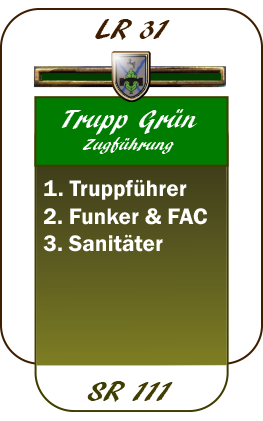
\includegraphics[width=0.3\textwidth]{./img/truppenordnung/zugfuehrung/zugfuehrung}
	%\caption{Beispiel eines \aclp{SQL}}
	\vspace{-50pt}
\end{wrapfigure}
Die Zugführung ist das Führungselement der Infanterie und Bindeglied zu den anderen Trupps. Einer Zugführung unterstellt sind typischerweise zwei, maximal drei Infanterietrupps, des weiteren kann ein Zug durch maximal einen Spezialtrupp mit klarer Aufgabenstellung unterstützt werden. Die Kommunikation zwischen dem Zugführer und der ihm untergeordneten Trupps erfolgt über Short-Range ohne Funkprotokoll über den sogenannten Zugkanal, die Kommunikation zu anderen Trupps über Long-Range.\\

Eine Zugführung besteht aus ein bis drei Spielern:
\begin{itemize}
	\item Zugführer\,/\,Squadlead (SQL)): Er befehligt die ihm untergeordneten Trupps. Ist kein Funker in der Zugführung vorhanden, übernimmt er auch die LR"=Kommunikation zu anderen Einheiten, in diesem Fall fällt jedoch die interne SR"=Truppfrequenz weg und der Zugfunk wird zum Standardfunk des Zugführers.
	\item Funker\,/\,Radio Operator (RO): Übernimmt die Kommunikation zu anderen Einheiten, damit der Zugführer sich auf die Führung seiner Truppen konzentrieren kann. Optional, wird jedoch dringend empfohlen.
	\item Gefechtssanitäter\,/\,Combat Medic (CM): Sanitäter für die Erstversorgung und Organisation der Verwundeten im Feld. Optional.
\end{itemize}
Sollten mehrere Züge im Verbund arbeiten, so einigen sich die Funker dieser Züge im Vorhinein auf eine sogenannte Task"=Force"=Frequenz, die sie sich auf der Additional"=Long"=Range einrichten und über die sie direkt ohne Funkprotokoll miteinander kommunizieren können (ähnlich wie der Zugkanal).\\
Die Zugführung sollte immer in Sichtweite der ihr unterstellten Trupps bleiben und sich maximal 200m bis 300m von ihnen entfernen, optimalerweise jedoch so nah wie möglich an ihren Truppen sein.